\section{The Universal Transformer }%: A Self-attentive Concurrent-Recurrent Sequence Model}
Here, in this section, we focus on the following research question:
\resq{c6.1}

The Universal Transformer (UT; see Figure~\ref{fig:universal-transformer-complete}) is based on the popular encoder-decoder architecture commonly used in most neural sequence-to-sequence models \citep{sutskever14,cho2014learning,transformer}. Both the encoder and decoder of the UT operate by applying a recurrent neural network to the representations of each of the positions of the input and output sequence, respectively. However, in contrast to most applications of recurrent neural networks to sequential data, the UT does not recur over positions in the sequence, but over consecutive revisions of the vector representations of each position (i.e., over ``depth''). In other words, the UT is not computationally bound by the number of symbols in the sequence, but only by the number of revisions made to each symbol's representation.

In each recurrent time-step, the representation of every position is concurrently (in parallel) revised in two sub-steps: first, using a self-attention mechanism to exchange information across all positions in the sequence, thereby generating a vector representation for each position that is informed by the representations of all other positions at the previous time-step. Then, by applying a transition function (shared across position and time) to the outputs of the self-attention mechanism, independently at each position. As the recurrent transition function can be applied any number of times, this implies that UTs can have variable depth (number of per-symbol processing steps). Crucially, this is in contrast to most popular neural sequence models, including the Transformer~\citep{transformer} or deep RNNs, which have constant depth as a result of applying a \emph{fixed stack} of layers.  We now describe the encoder and decoder in more detail (See Figure~\ref{fig:universal-transformer-complete} for the schema of the complete model.).

\begin{figure}[t]
 \centering
 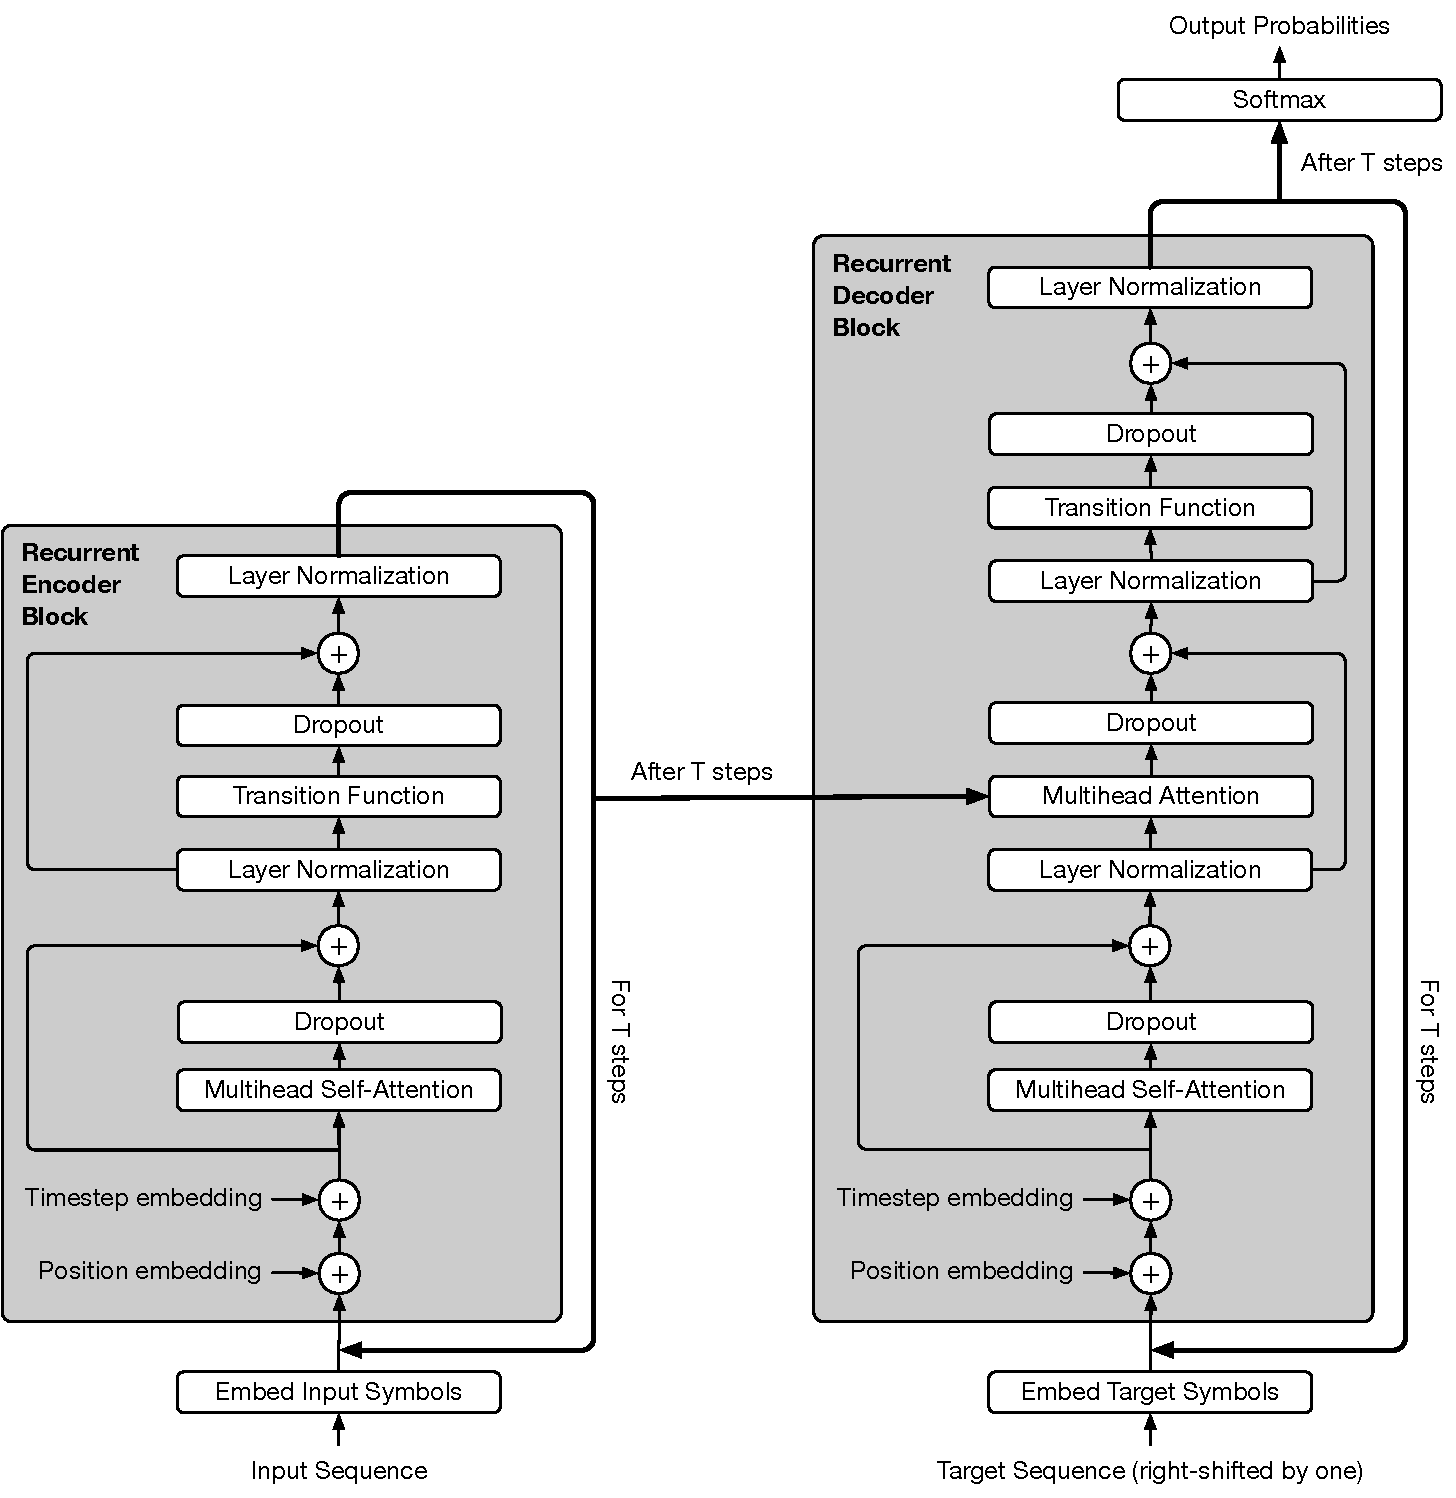
\includegraphics[width=0.9\textwidth]{04-part-03/chapter-06/figs_and_tables/fig_universal-transformer-complete.pdf}
 \caption{The recurrent blocks of the Universal Transformer encoder and decoder.}
 \label{fig:universal-transformer-complete}
\end{figure}

\subsubsection{\textsc{Encoder:}}
Given an input sequence of length $m$, we start with a matrix whose rows are initialized as the $d$-dimensional embeddings of the symbols at each position of the sequence $H^0 \in \mathbb{R}^{m \times d}$. The UT then iteratively computes representations $H^t$ at step $t$ for all $m$ positions in parallel by applying the multi-headed dot-product self-attention mechanism from \cite{transformer}, followed by a recurrent transition function. We also add residual connections around each of these function blocks and apply dropout and layer normalization \citep{srivastava2014dropout, layernorm2016}.

Before describing the details of the first block of the universal transformer, i.e., the multi-head attention, we explain the attention mechanism in general as the main building block of many of state-of-the-art models.
An attention mechanism is usually based on a memory-query paradigm. In this setup, there exist a memory $M$ that contains a collection of items, each representing information from a source modality (like the hidden state of the encoder), and a query $q$ vector that contains information from a target modality (like the hidden state of the decoder).\footnote{In self-attention, queries and memory are from the same modality.}
Each item in the memory is associated with a key and value ($k_i$, and $v_i$), where the key is used to compute the probability that indicates how well the query matches the item:
\begin{equation}
a_i = \frac{exp(f_{\text{att}}(q, k_i)}{\sum_{j=1}^|M| exp(f_{\text{att}}(q, k_j)},
\end{equation}
where the $f_\text{att}$ can be the dot product function~\citep{luong2015effective} or a multilayer perceptron~\citep{bahdanau2014neural}. Then, given the attention distributions over all items in the memory which is calculated by querying the memory with query $q$, we can output a value that is a sum over all the values in the memory weighted by their probabilities, which can  be fed to other parts of the model for further calculation.

In the Universal Transformer, similar to the Transformer, we use the scaled dot-product attention which combines queries $Q$, keys $K$ and values $V$ as follows

\begin{equation}
   \textsc{Attention}(Q, K, V) = \textsc{softmax} \left( \frac{QK^T}{\sqrt{d}} \right) V,
\end{equation}

where $d$ is the number of columns of $Q$, $K$ and $V$. We use the multi-head version with $k$ heads, as introduced in \citep{transformer}:
\begin{align}
    \label{MultiheadSelfAttention}
    \textsc{MultiHeadSelfAttention}(H^t) &= \textsc{Concat}(\mathrm{head_1}, ..., \mathrm{head_k})W^O\\
    \text{where}~\mathrm{head_i} &= \textsc{Attention}(H^t W^Q_i, H^t W^K_i, H^t W^V_i),
\end{align}
and we map the state $H^t$ to queries, keys and values with affine projections using learned parameter matrices $W^Q \in \mathbb{R}^{d \times d/k}$, $W^K \in \mathbb{R}^{d \times d/k}$, $W^V \in \mathbb{R}^{d \times d/k}$ and $W^O \in \mathbb{R}^{d \times d}$.

At step $t$, the UT then computes revised representations $H^t \in \mathbb{R}^{m \times d}$ for all $m$ input positions as follows:
\begin{align}
    \label{RecurrentTransition}
    H^t &= \textsc{LayerNorm}(A^{t} + \textsc{Transition}(A^t) ) \\
    \mathrm{where}~A^t &= \textsc{LayerNorm}((H^{t-1} + P^{t}) + \\ 
    &  \textsc{MultiHeadSelfAttention}(H^{t-1} + P^{t})),
\end{align}
where \textsc{LayerNorm()} is defined in \cite{layernorm2016}, and \textsc{Transition()} and $P^t$ are discussed below.

Depending on the task, we use one of two different transition functions: either a separable convolution~\citep{xception2016} or a fully-connected neural network that consists of a single rectified-linear activation function between two affine transformations, applied position-wise, i.e., individually to each row of $A^t$.

$P^t \in \mathbb{R}^{m \times d}$ above are fixed, constant, two-dimensional (position, time) \emph{coordinate embeddings}, obtained by computing the sinusoidal position embedding vectors as defined in \citep{transformer} for the positions $1 \leq i \leq m$ and the time-step $1 \leq t \leq T$ separately for each vector-dimension $1 \leq j \leq d$, and summing:
\begin{align}
\label{eqn:coordinate-embeddings}
    P^t_{i, 2j} &= \sin(i / 10000^{2j / d}) + \sin(t / 10000^{2j / d}) \\
    P^t_{i, 2j+1} &= \cos(i / 10000^{2j / d}) + \cos(t / 10000^{2j / d}).
\end{align}

After $T$ steps (each updating all positions of the input sequence in parallel), the final output of the Universal Transformer encoder is a matrix of $d$-dimensional vector representations $H^T \in \mathbb{R}^{m \times d}$\footnote{Note that $T$ in $H^T$ denotes time-step $T$ and not the transpose operation.} for the $m$ symbols of the input sequence.

\subsubsection{\textsc{Decoder:}}
The decoder shares the same basic recurrent structure of the encoder. However, after the self-attention function, the decoder additionally also attends to the final encoder representation $H^T$ of each position in the input sequence using the same multihead dot-product attention function from Equation \ref{MultiheadSelfAttention}, but with queries $Q$ obtained from projecting the \emph{decoder} representations, and keys and values ($K$ and $V$) obtained from projecting the \emph{encoder} representations (this process is akin to standard attention \citep{bahdanau2014neural}).

Like the Transformer model, the UT is autoregressive \citep{graves2013generating}. Trained using teacher-forcing, at generation time it produces its output one symbol at a time, with the decoder consuming the previously produced output positions. During training, the decoder input is the target output, shifted to the right by one position.
The decoder self-attention distributions are further masked so that the model can only attend to positions to the left of any predicted symbol. Finally, the per-symbol target distributions are obtained by applying an affine transformation $O \in \mathbb{R}^{d \times V}$ from the final decoder state to the output vocabulary size $V$, followed by a softmax which yields an $(m \times V)$-dimensional output matrix normalized over its rows:
\begin{equation}
 p\left(y_{pos} | y_{[1:pos - 1]}, H^T\right) = \textsc{softmax}(OH^T)
\end{equation}

To generate from the model, the encoder is run once for the conditioning input sequence. Then the decoder is run repeatedly, consuming all already-generated symbols, while generating one additional distribution over the vocabulary for the symbol at the next output position per iteration. We then typically sample or select the highest probability symbol as the next symbol.


\subsection{Adaptive Computation by Dynamic Halting}
\label{sec:dynamic-halting}
\begin{figure}
 \centering
 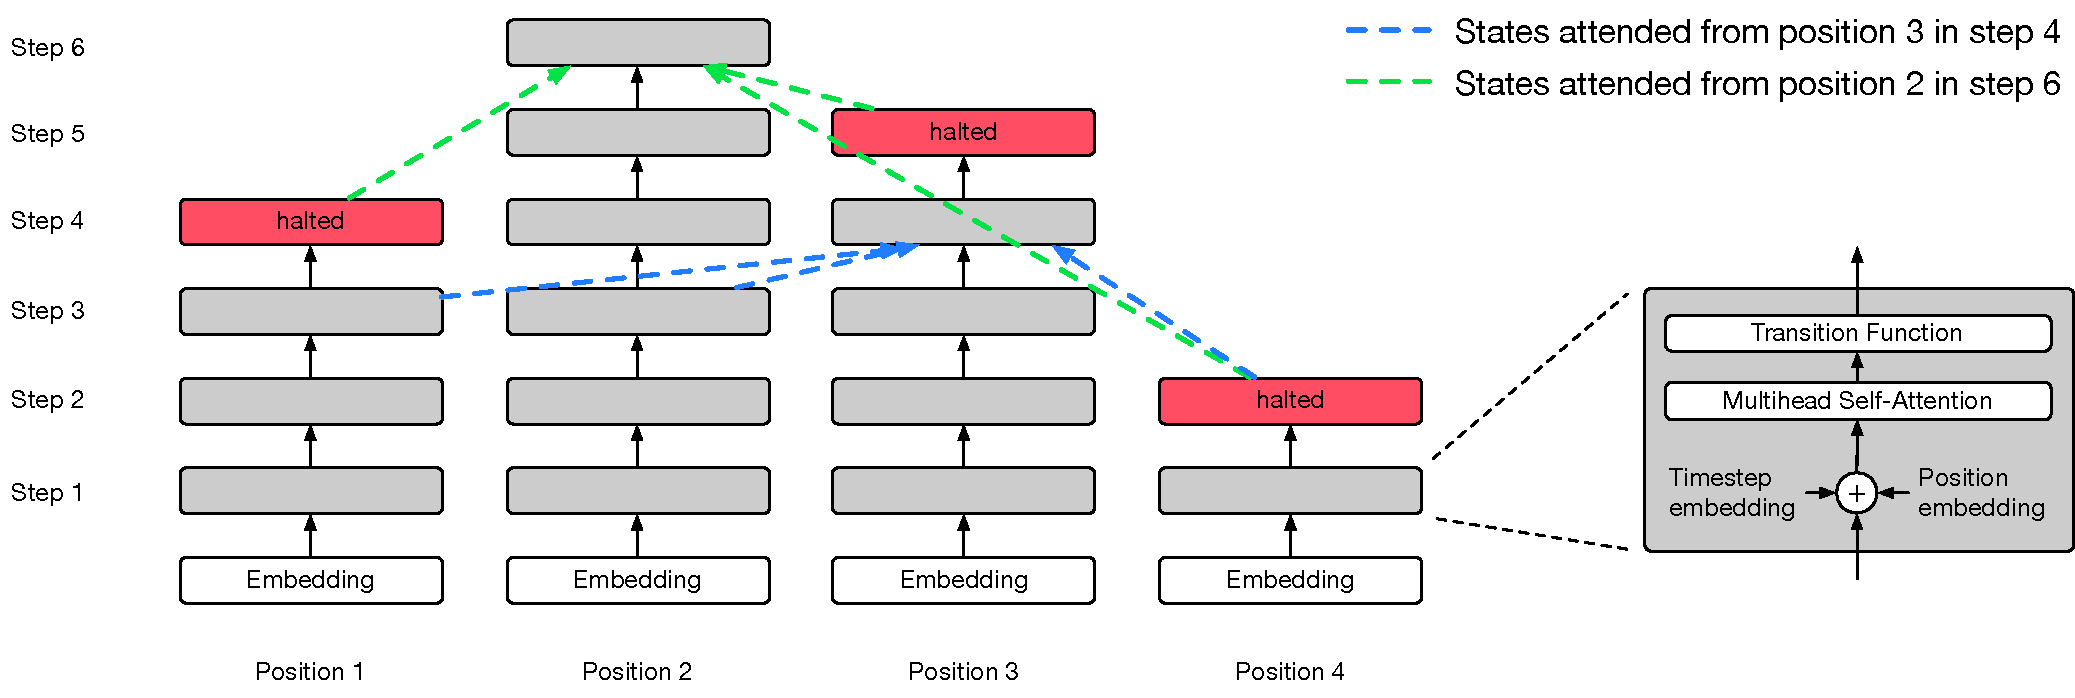
\includegraphics[width=1.0\textwidth]{04-part-03/chapter-06/figs_and_tables/fig_adaptive-universal-transformer.pdf}
 \caption{An unrolled visualization of Universal Transformer with dynamic halting. It illustrates different numbers of recurrent revisions per position (best viewed in colour).}
 \label{fig:adaptive_ut}
\end{figure}
In sequence processing systems, certain symbols (e.g., some words or phonemes) are usually more ambiguous than others. It is therefore reasonable to allocate more processing resources to these more ambiguous symbols. Adaptive Computation Time (ACT) \citep{graves2016adaptive} is a mechanism for dynamically modulating the number of computational steps needed to process each input symbol (called the ``ponder time'') in standard recurrent neural networks based on a scalar \emph{halting probability} predicted by the model at each step.

Inspired by the interpretation of Universal Transformers as applying self-attentive RNNs in parallel to all positions in the sequence, we also add a dynamic ACT halting mechanism to each position, i.e., to each per-symbol self-attentive RNN. Once the per-symbol recurrent block halts, its state is simply copied to the next step until all blocks halt, or we reach a maximum number of steps. The final output of the encoder is then the final layer of representations produced in this way. Figure~\ref{fig:adaptive_ut} illustrates a Universal Transformer encoder with $T$, number of revisions, dynamically determined for each position.


We implement dynamic halting based on ACT~\citep{graves2016adaptive}. In each step of the UT with dynamic halting, we are given the halting probabilities, remainders, number of updates up to that point, and the previous state (all initialized as zeros), as well as a scalar threshold between 0 and 1 (a hyper-parameter). We then compute the new state for each position and calculate the new per-position halting probabilities based on the state for each position.\footnote{The current implementation of adaptive computation time does not allow for a fully end-to-end backpropable gradient of the proposed training loss. However, the discontinuity of the cost function might not imply that meaningful learning is not possible and in fact, the experiments in the original paper~\citep{graves2016adaptive} as well as here in Universal Transformer with adaptive halting suggest it works fine.} The UT then decides to halt for some positions that crossed the threshold, and updates the state of other positions until the model halts for all positions or reaches a predefined maximum number of steps. 
The following is a simplified TensorFlow~\citep{tensorflow2015-whitepaper} code that shows the details for the adapted ACT mechanism.
\begin{lstlisting}[language=Python, caption=UT with dynamic halting.]
# While-loop stops when this predicate is FALSE
# i.e. all ((probability < threshold) & (counter < max_steps)) are false
def should_continue(u0, u1, halting_probability, u2, n_updates, u3):
return tf.reduce_any(
            tf.logical_and(
                tf.less(halting_probability, threshold),
                tf.less(n_updates, max_steps)))
# Do while loop iterations until predicate above is false
(_, _, _, remainder, n_updates, new_state) = tf.while_loop(
    should_continue, ut_with_dynamic_halting, (state, 
    step, halting_probability, remainders, n_updates, previous_state))
\end{lstlisting}


% \begin{lstlisting}[language=Python, caption=]
%  # initializing halting probabilities
% halting_probability = tf.zeros(
%   (
%       batch_size,
%       length,
%   ), name="halting_probability")
% # initializing remainders 
% remainders = tf.zeros(
%   (
%       batch_size,
%       length,
%   ), name="remainder")
% # initializing number of updates performed 
% n_updates = tf.zeros(
%   (
%       batch_size,
%       length,
%   ), name="n_updates")

% # initializing Previous cell states
% previous_state = tf.zeros_like(state, name="previous_state")
% step = tf.constant(0, dtype=tf.int32)

% # While loop stops when this predicate is FALSE.
% # Ie all (probability < 1-eps AND counter < N) are false.
% def should_continue(u0, u1, halting_probability, u2, n_updates, u3):
% return tf.reduce_any(
%     tf.logical_and(
%         tf.less(halting_probability, threshold),
%         tf.less(n_updates, act_max_steps)))

% # Do while loop iterations until predicate above is false.
% (_, _, _, remainder, n_updates, new_state) = tf.while_loop(
%   should_continue, ut_with_dynamic_halting,
%   (state, step, halting_probability, remainders, n_updates, previous_state))
% \end{lstlisting}


The following shows the computations in each step:

\begin{lstlisting}[language=Python, caption=Computations in each step of the UT with dynamic halting.]
def ut_with_dynamic_halting(state, step, halting_probability, 
                            remainders, n_updates, previous_state):
    # Calculate the probabilities based on the state 
    p = common_layers.dense(state, 1, activation=tf.nn.sigmoid, 
        use_bias=True)
    # Mask for inputs which have not halted yet
    still_running = tf.cast(
        tf.less(halting_probability,1.0), tf.float32)
    # Mask of inputs which halted at this step
    new_halted = tf.cast(
        tf.greater(halting_probability + p * still_running, threshold), 
            tf.float32) * still_running
    # Mask of inputs which haven't halted, and didn't halt this step
    still_running = tf.cast(
        tf.less_equal(halting_probability + p * still_running, 
            threshold), tf.float32) * still_running
    # Add the halting probability for this step to the halting
    # probabilities for those inputs which haven't halted yet
    halting_probability += p * still_running
    # Compute remainders for the inputs which halted at this step
    remainders += new_halted * (1 - halting_probability)
    # Add the remainders to those inputs which halted at this step
    halting_probability += new_halted * remainders
    # Increment n_updates for all inputs which are still running
    n_updates += still_running + new_halted
    # Compute the weight to be applied to the new state and output:
    #   0 when the input has already halted,
    #   p when the input hasn't halted yet,
    #   the remainders when it halted this step.
    update_weights = tf.expand_dims(p * still_running +
                                    new_halted * remainders, -1)
    # Apply transformation to the state
    transformed_state = transition_function(self_attention(state))
    # Interpolate transformed and previous states for non-halted inputs
    new_state = ((transformed_state * update_weights) +
                 (previous_state * (1 - update_weights)))
    step += 1
    return (transformed_state, step, halting_probability,
            remainders, n_updates, new_state)
\end{lstlisting}


\section{Universality and Relation to other Models}
\label{sec:related}
When running for a fixed number of steps, the Universal Transformer is equivalent to a multi-layer Transformer with tied parameters across all its layers. This is partly similar to the Recursive Transformer, which ties the weights of its self-attention layers across depth~\citep{gulcehre2018hyperbolic}.\footnote{Note that in UT both the self-attention and transition weights are tied across layers.} However, as the per-symbol recurrent transition functions can be applied any number of times, another and possibly more informative way of characterizing the UT is as a block of parallel RNNs (one for each symbol, with shared parameters) evolving per-symbol hidden states concurrently, generated at each step by attending to the sequence of hidden states at the previous step. In this way, it is related to architectures such as the Neural GPU \citep{neural_gpu} and the Neural Turing Machine \citep{ntm14}. UTs thereby retain the attractive computational efficiency of the original feed-forward Transformer model, but with the added recurrent inductive bias of RNNs. Furthermore, using a dynamic halting mechanism, UTs can choose the number of processing steps based on the input data. %interpolate between the feed-forward, fixed-depth Transformer and a gated, recurrent architecture running for a number of steps dependent on the input data. 

The connection between the Universal Transformer and other sequence models is apparent from the architecture: if we limited the recurrent steps to one, it would be a Transformer. But it is more interesting to consider the relationship between the Universal Transformer and RNNs and other networks where recurrence happens over the time dimension. Superficially these models may seem closely related since they are recurrent as well. But there is a crucial difference: time-recurrent models like RNNs cannot access memory in the recurrent steps. This makes them computationally more similar to automata, since the only memory available in the recurrent part is a fixed-size state vector. UTs, on the other hand, can attend to the whole previous layer, allowing it to access memory in the recurrent step. 

Given sufficient memory the Universal Transformer is computationally universal -- i.e., it belongs to the class of models that can be used to simulate any Turing machine, thereby addressing a shortcoming of the standard Transformer model. In addition to being theoretically appealing, our results show that this added expressivity also leads to improved accuracy on several challenging sequence modeling tasks. This closes the gap between practical sequence models competitive on large-scale tasks such as machine translation, and computationally universal models such as the Neural Turing Machine or the Neural GPU \citep{ntm14,neural_gpu}, which can be trained using gradient descent to perform algorithmic tasks.

To show this, we can reduce a Neural GPU to a Universal Transformer. Ignoring the decoder and parameterizing the self-attention module, i.e., self-attention with the residual connection, to be the identity function, we assume the transition function to be a convolution. If we now set the total number of recurrent steps $T$ to be equal to the input length, we obtain exactly a Neural GPU. Note that the last step is where the Universal Transformer crucially differs from the vanilla Transformer whose depth cannot scale dynamically with the size of the input. A similar relationship exists between the Universal Transformer and the Neural Turing Machine, whose single read/write operations per step can be expressed by the global, parallel representation revisions of the Universal Transformer. In contrast to these models, however, which only perform well on algorithmic tasks, the Universal Transformer also achieves competitive results on realistic natural language tasks such as LAMBADA and machine translation.

Another related model architecture is that of end-to-end Memory Networks \citep{sukhbaatar2015}. In contrast to end-to-end memory networks, however, the Universal Transformer uses memory corresponding to states aligned to individual positions of its inputs or outputs. Furthermore, the Universal Transformer follows the encoder-decoder configuration and achieves competitive performance in large-scale sequence-to-sequence tasks.


\subsection{On the Computational Power of UT vs Transformer}
\label{app:univerrality_example}

With respect to their computational power, the key difference between the Transformer and the Universal Transformer lies in the number of sequential steps of computation (i.e., in depth). While a standard Transformer executes a total number of operations that scales with the input size, the number of sequential operations is constant, independent of the input size and determined solely by the number of layers. Assuming finite precision, this property implies that the standard Transformer cannot be computationally universal. When choosing a number of steps as a function of the input length, however, the Universal Transformer does not suffer from this limitation. Note that this holds independently of whether or not adaptive computation time is employed but does assume a non-constant, even if possibly deterministic, number of steps. Varying the number of steps dynamically after training is enabled by sharing weights across sequential computation steps in the Universal Transformer.

\begin{figure}[t]
\centering
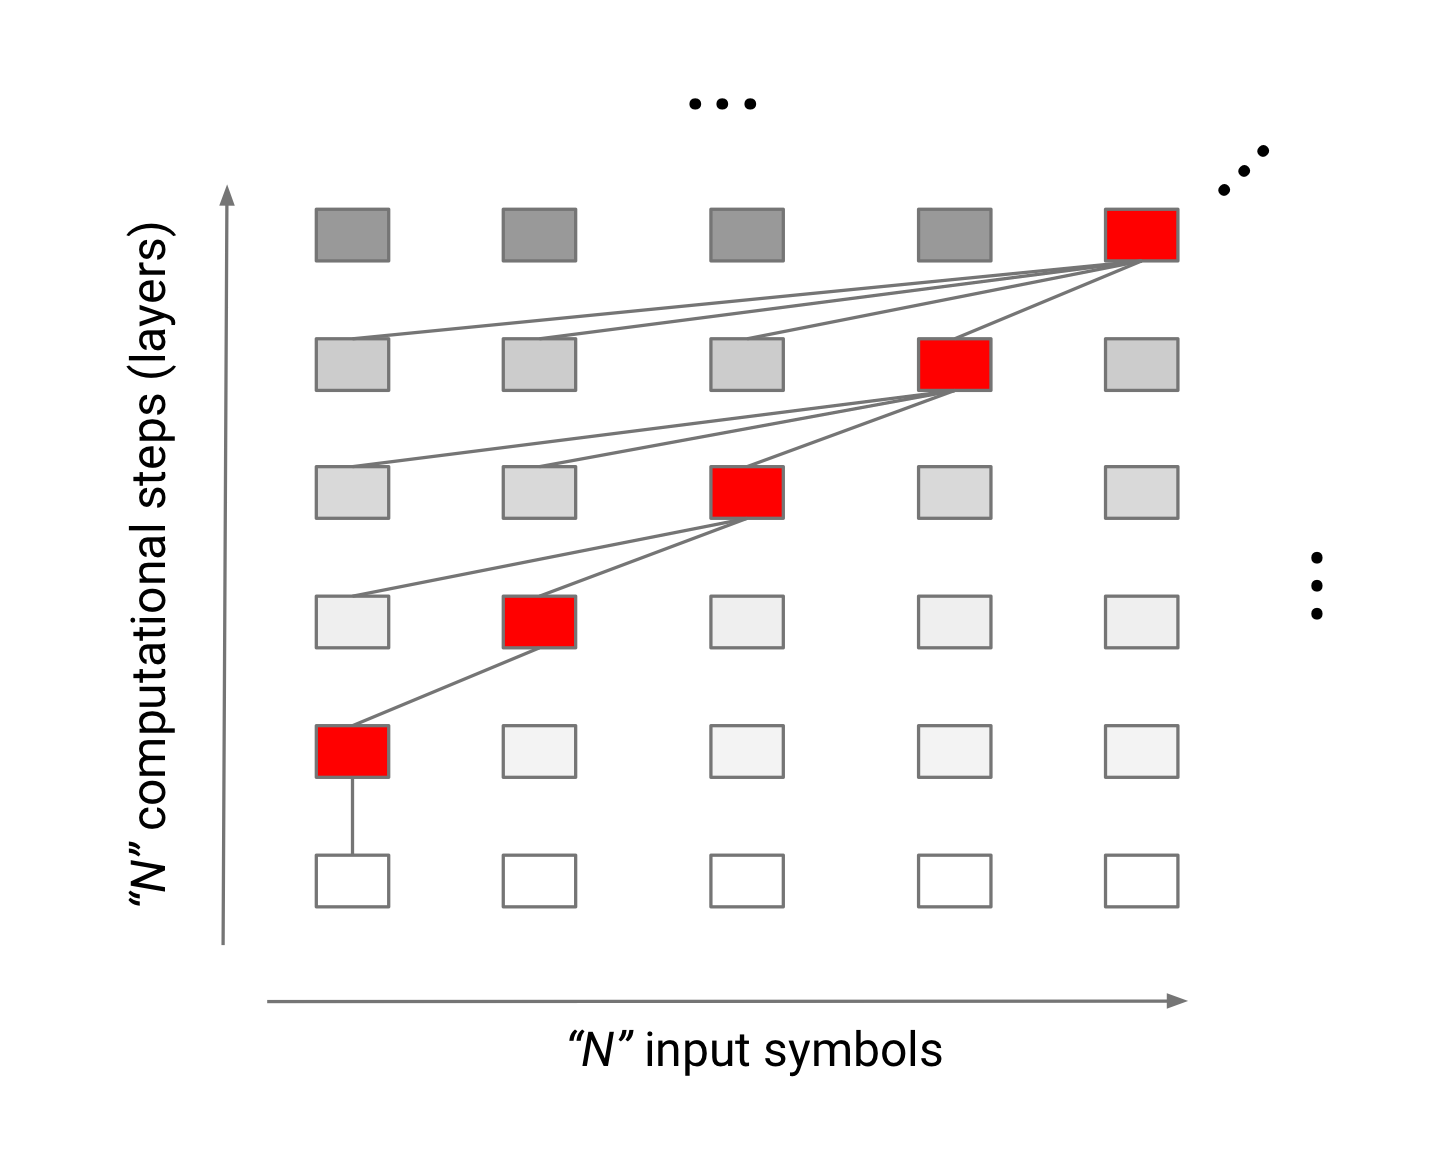
\includegraphics[width=0.7\textwidth, trim={0.1cm 0.5cm 0.1cm 1.2cm}, clip]{04-part-03/chapter-06/figs_and_tables/fig_universality_example.png}
\end{figure}

An intuitive example are functions whose execution requires the sequential processing of each input element. In this case, for any given choice of depth $T$, one can construct an input sequence of length $N>T$ that cannot be processed correctly by a standard Transformer. With an appropriate, input-length dependent choice of sequential steps, however, a Universal Transformer, RNNs or Neural GPUs can execute such a function.